\lesson{2}{Apr 06 2022 Wed (07:25:34)}{Angles and Arc-Length}
\label{les_2:angles_and_arc_length}

\begin{figure}[htpb]
  \centering

  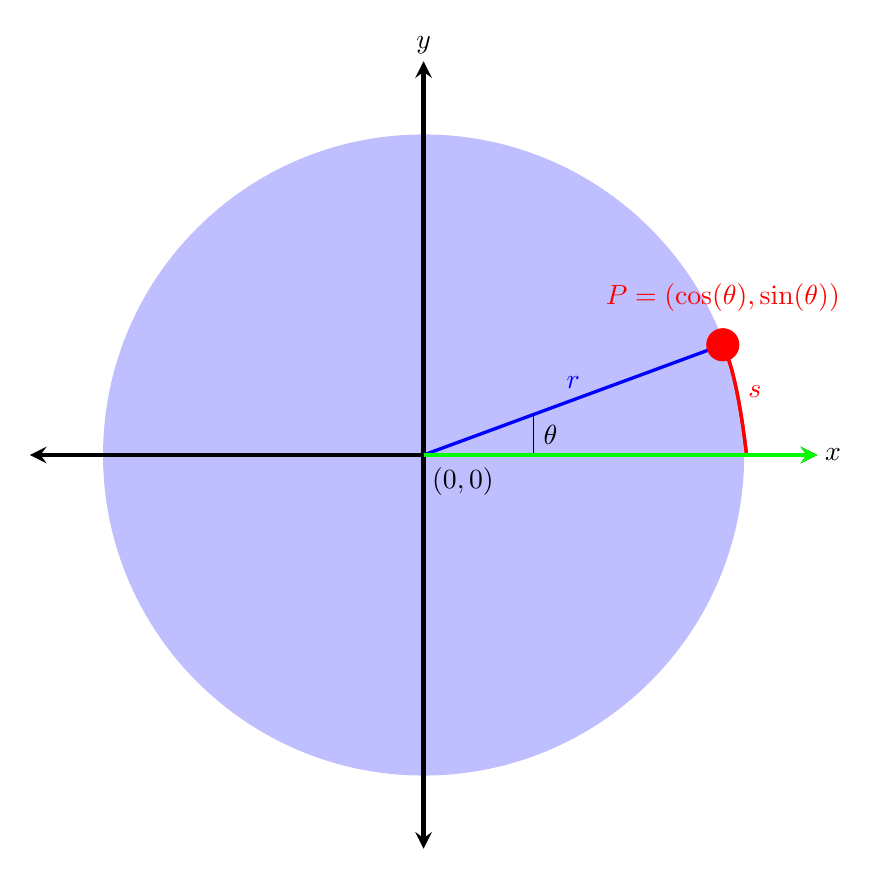
\begin{tikzpicture}
    \coordinate (O) at (0,0);

    \draw[draw=blue!25!white,fill=blue!25!white] (O) circle (1.60in);

    \draw (0.50,-0.04) node[fill=blue!25!white,anchor=north] {$(0,0)$};
    \draw (0,5.2) node[fill=white,anchor=center] {$y$};
    \draw (5.2,0) node[fill=white,anchor=center] {$x$};

    \draw[stealth-stealth,ultra thick] (0,5) -- (0,-5);
    \draw[stealth-stealth,ultra thick] (5,0) -- (-5,0);

    \draw[blue,very thick] (0,0) to node[anchor=south] {$r$} (3.8,1.4);
    \draw[draw=red,fill=red] (3.8,1.4) circle (0.08in);
    \draw[red] (3.8,2) node[anchor=center] {$P = (\cos (\theta), \sin (\theta))$};
    \draw[very thick,red] (3.8,1.4) arc (74:39:0.6cm and 4.2cm);

    \draw (1.4,0.52) to node[right] {$\theta$} (1.4,0);

    \draw[very thick,red] (3.8,1.4) arc (74:39:0.6cm and 4.2cm);
    \draw[red] (4,0.8) node[anchor=west] {$s$};
    \draw[ultra thick,green,-stealth] (0,0) -- (5,0);
  \end{tikzpicture}

  \caption{Diagram of a Circle}
  \label{fig:circle_diagram}
\end{figure}

\begin{itemize}
  \label{item:angles_and_arc_length}

  \item The standard way that we put an angle in a circle we
    start the angle at the positive $x$-axis and go \textbf{counterclockwise}.
    We measure negative angles \textbf{clockwise}.
  \item When put an angle in standard position and you rotate,
    it ends someplace. Where it ends is called the \textbf{Terminal Side}.
  \item The point $P$ on the circumference of the circle is
    \textbf{specified by the angle} $\theta$.
  \item Angle $\theta$ corresponds with a portion of the
    circumference of the circle called the \textbf{arc spanned by $\theta$}
  \item Two angles with the same terminal side are called
    \textbf{co-terminal angles}.
\end{itemize}

Three hundred and sixty degrees ($360^{\circ}$) represents a complete trip
around a circle, which is a full rotation. So, $1^{\circ}$ corresponds to 
$\frac{1}{360^{\circ}}$ of a full rotation. Degrees are more like percentages,
where they represent concepts, and not numbers. But, just like how you can
transform a percentage to a number ($10 \% = \frac{10}{100}$), you can do the
same with degrees ($10^{\circ} = \frac{10}{360}$).

Since $360^{\circ}$ represents a full rotation around the circle, if we add any
integer multiple of $360^{\circ}$ to an angle $\theta_1$, we'll obtain an angle
co-terminal to $\theta_1$.

\begin{example}
  \label{exm:co_terminal_to_theta}

  So $45^{\circ}$ and $405^{\circ}$ are co-terminal.
\end{example}

\begin{definition}[$\pi$]
  \label{def:pi}

  The number $\pi$ represents the ratio of the circumference of a circle to the
  diameter of the circle. $\pi = \frac{c}{d}$, where $c$ is the circumference
  and $d$ is the diameter.
  
  $\pi \approx 3.14$, but $\pi$ is an \textbf{"irrational"} number.
\end{definition}

\begin{definition}[Radian]
  \label{def:radion}

  The \textbf{radian} measure of an angle is the ratio of the length of the arc
  on the circumference of the circle spanned by the angle, $s$, and the radius,
  $r$, of the circle.

  \begin{equation*}
    \label{edt:entire_revolution_using_raidans}
    \begin{alignedat}{3}
      \theta &= \frac{s}{r} \\
      \pi &= \frac{c}{d} \\
          &= \frac{2}{2r} \qquad && \textrm{$d = 2r$} \\
      2\pi &= \frac{c}{r} \qquad && \textrm{Multiply both sides by $2$} \\
    \end{alignedat}
  .\end{equation*}

  From this, we can conclude that: $2\pi = 360^{\circ}$. From that, we can get
  $\pi = 180^{\circ}$ since we just divided both sides by $2$. From that, we get
  $\frac{\pi}{2} = 90^{\circ}$. So on, and so forth.

  Here's a table with all of the radians:

  \begin{table}[H]
    \label{tab:degrees_into_radians}
    \centering

    \begin{tabular}{|c|c|c|c|c|c|c|c|c|}
      \hline
      $\theta$ (degrees) & $0^{\circ}$ & $30^{\circ}$ & $45^{\circ}$ & $60^{\circ}$ & $90^{\circ}$ & $180^{\circ}$ & $270^{\circ}$ & $360^{\circ}$ \\
      \hline
      $\theta$ (radians) & $0$ & $\frac{\pi}{6}$ & $\frac{\pi}{4}$ &
      $\frac{\pi}{3}$ & $\frac{\pi}{2}$ & $\pi$ & $\frac{3\pi}{2}$ & $2\pi$ \\
      \hline
    \end{tabular}

    \caption{Degrees into Radians}
  \end{table}
\end{definition}

\begin{exc}[Solution \ref{sol:convert_8_radians_into_degrees_and_8_into_radians}]
  \label{exc:convert_8_radians_into_degrees_and_8_into_radians}

  Convert $8$ radians into degrees and $8$ degrees into radians:
\end{exc}

\begin{definition}[Arc Length]
  \label{def:arc_length}

  The \textbf{arc length} $s$ spanned in a circle of radius $r$ by an angle
  $\theta$ measured in radians is given by:
  \[ s = r \times \mid \theta \mid \].

  \begin{note}
    This formula only applies if $\theta$ is measured in radians.
  \end{note}
\end{definition}

\begin{exc}[Solution \ref{sol:what_is_the_arc_length_spanned_by_a_40_degree_angle_on_a_circle_of_radius_30_meters}]
  \label{exc:what_is_the_arc_length_spanned_by_a_40_degree_angle_on_a_circle_of_radius_30_meters}

  What is the arc length spanned by a $40^{\circ}$ angle on a circle radius $30$
  meters?
\end{exc}

\newpage
